\documentclass[10pt,a4paper]{paper}

\usepackage[latin1]{inputenc}
\usepackage[english]{babel}

\usepackage[official,right]{eurosym}
\usepackage{hyperref}
\usepackage{graphicx}
\usepackage{a4wide}
\usepackage{calc}
%\usepackage{picins}
\usepackage{fancyhdr}
\usepackage{amssymb,amsmath}
\usepackage{gensymb}
%\usepackage{multicol}
\usepackage{url}



% For drawings
\usepackage{pgf}
\usepackage{tikz}
\usetikzlibrary{arrows,automata}
\usepackage{color}

% For quick and easy figures
\newcommand{\pic}[3]{
\begin{figure}[h]\begin{center}\includegraphics[width=#2]{#1.png} 
	\caption{#3}
	\label{#1}
\end{center}\end{figure}
}

%\newcommand{\inHfile}[2]{
%	Function \texttt{#1} in File \texttt{#2.h} \\
%}
%\newcommand{\inCfile}[2]{
%	Function \texttt{#1} in File \texttt{#2.c} \\
%}

\newcommand{\inHfile}[2]{Function \texttt{#1}\\
\indent in File \texttt{#2.h} \\}

\newcommand{\inCfile}[2]{Function \texttt{#1}\\
\indent in File \texttt{#2.c} \\}

%\numberwithin{equation}{section}
\newcommand{\vect}[1]{\ensuremath{\overrightarrow{#1}}}		%% How to mark Vectors
\newcommand{\eu}[1]{\ensuremath{#1^{\phi}}}			%% how to mark euler angles
\newcommand{\ra}[1]{\ensuremath{\omega_{#1}}}		%% how to mark rates
\newcommand{\ew}[1]{\;. \! \!#1}					%% how to mark element-wise operations
\newcommand{\mat}[1]{\ensuremath{\mathbf{#1}}}		%% how to mark Matrices
\newcommand{\eye}[0]{\mat{I}}						%% Identity matrix
\newcommand{\quat}[1]{\ensuremath{q_{#1}}}			%% how to mark Quaternions
\newcommand{\transp}[1]{\ensuremath{#1^{T}}}
\newcommand{\est}[1]{\ensuremath{\hat{#1}}}
\newcommand{\err}[1]{\ensuremath{\tilde{#1}}}
\newcommand{\meas}[1]{\ensuremath{\tilde{#1}}}
\newcommand{\linpt}[1]{\ensuremath{\overline{#1}}}
\newcommand{\norm}[1]{\ensuremath{\Vert{#1}\Vert}}
\newcommand{\quatprod}[0]{\ensuremath{\bullet}}
\newcommand{\ddt}[2]{\ensuremath{#1^{(#2)}}}
\newcommand{\deriv}[2]{\ensuremath{{#1}^{(#2)}}}
\newcommand{\inv}[1]{\ensuremath{#1}^{-1}}
\newcommand{\comp}[1]{\ensuremath{#1}^*}
\newcommand{\atan}[1]{\ensuremath{\text{atan}\left({#1}\right)}}
\newcommand{\sign}[1]{\ensuremath{\text{sign}\left({#1}\right)}}
\newcommand{\cross}{\ensuremath{\times}}

\newcommand{\division}[0]{\ensuremath{\div}}
\newcommand{\multiplication}[0]{\ensuremath{\cdot}}


%% Formatting in the right color for euler angles
\definecolor{rollcolor}{rgb}{0,0,1}
\definecolor{pitchcolor}{rgb}{0,0.5,0}
\definecolor{yawcolor}{rgb}{1,0,0}
\newcommand{\Rollc}[1]{\color{rollcolor}#1\color{black}{}}
\newcommand{\Pitchc}[1]{\color{pitchcolor}#1\color{black}{}}
\newcommand{\Yawc}[1]{\color{yawcolor}#1\color{black}{}}
\newcommand{\Roll}[0]{\ensuremath{\Rollc \phi}}
\newcommand{\Pitch}[0]{\ensuremath{\Pitchc \theta }}
\newcommand{\Yaw}[0]{\ensuremath{\Yawc \psi}}
\newcommand{\lon}[0]{\ensuremath{\lambda}}
\newcommand{\lat}[0]{\ensuremath{\varphi}}


\newcommand{\mynote}[1]{\begin{flushright}\fbox{Martin: ``\textit{#1}''}\end{flushright}}
%\newcommand{\mynote}[1]{}

\graphicspath{{./images/},{tmp/}}

\title{Documentation for pprz_algebra}
\author{Martin Dieblich}

\begin{document}

%\maketitle
This file is just a bunch of random stuff and notes for myself (and others, of course).
\section{ENU to NED transformations}
I had the problem very often that I have to transform form ENU no NED. The simple conversion: ``Flip x and y and negate z'' doesn't work for quaternions or if you want to use matrix algebra.

\subsection{Matrix}
Flipping x and y and negating z is easy to express as a matrix:
\begin{equation}
R_{ENU2NED} = \begin{pmatrix}
0 & 1 &  0 \\
1 & 0 &  0 \\
0 & 0 & -1
\end{pmatrix}
\end{equation}
This works in both directions, since $ R_{ENU2NED} = \transp R_{ENU2NED} $.

\subsection{Quaternion}
It's easy to compute a quaternion out of the above rotation matrix.
\begin{equation}
\quat{ENU2NED} = \frac{1}{\sqrt 2} \begin{pmatrix}
0 \\ 1 \\ 1 \\ 0
\end{pmatrix} = \frac{1}{\sqrt 2} (i + j)
\end{equation}
This makes sense, since the real value = 0 represents a rotation about $180^{\circ}$ and the three values for the axis $ \vect v = \transp{\begin{pmatrix}1&1&0\end{pmatrix}}$ represent the axis of rotation.

\subsubsection*{Transforming a quaternion between ENU/NED}
If you want to cahnge a quaternion from NED to ENU or vice versa. It's not totally simple like for vectors. \\
If your quaternion consist of the values:
\begin{equation}
\quat{ECEF2NED} = \begin{pmatrix}a \\ b \\ c\\d\end{pmatrix}
\end{equation}
Then a transformation to ENU (NED) is made as following:
\begin{equation}
\quat{ECEF2NED} = \frac{1}{\sqrt 2} \begin{pmatrix}-b-c \\ a+d \\ a-d\\-b+c\end{pmatrix}
\end{equation}

Pay attention doing it twice! The multiplication of an NED to ENU quaternion with itself leads to
\begin{equation}
\quat{ECEF2NED} \quatprod \quat{ECEF2NED} \quatprod \begin{pmatrix}a \\ b \\ c\\d\end{pmatrix}= \begin{pmatrix}-a \\ -b \\ -c\\-d\end{pmatrix} .
\end{equation}
This is logically the same rotation, but mathemaically a different quaternion. So don't be confused if all values are negative :-)

\section{Initialisation}

\subsection{What about the standard deviation?}
Pay attention to the following equations! Many things are just guesses and no really mathematically proofen. So better think twice before just using my assumptions.
\begin{figure}[h!]\begin{center}
	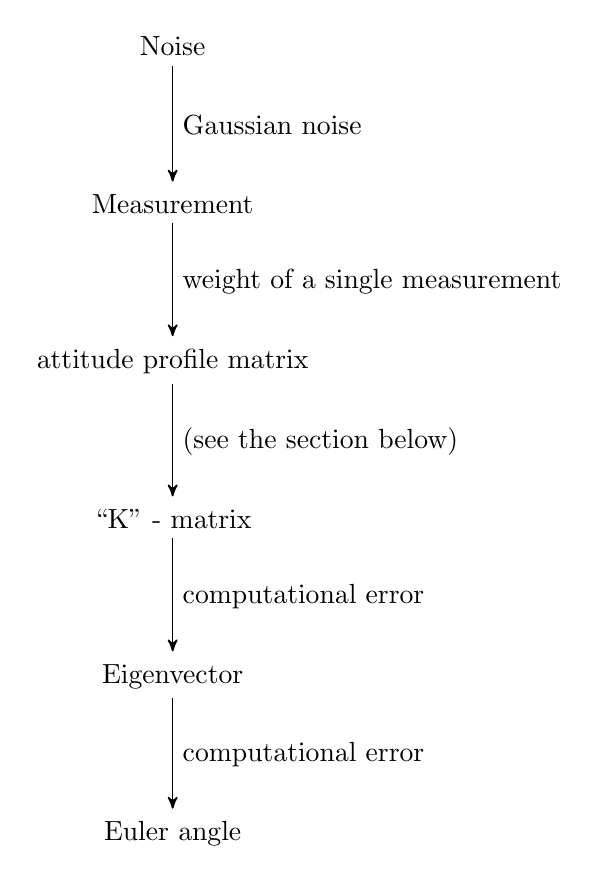
\begin{tikzpicture}[->,>=stealth',shorten >=1pt,auto,node distance=2cm,
                    semithick]
  \tikzstyle{every state}=[draw=black,text=white]

  \node		   (A)              {Noise};
  \node        (B) [below of=A] {Measurement};
  \node        (C) [below of=B] {attitude profile matrix};
  \node        (D) [below of=C] {``K'' - matrix};
  \node        (E) [below of=D] {Eigenvector};
  \node        (F) [below of=E] {Euler angle};

  \path (A) edge              node {Gaussian noise} (B)
  		(B) edge              node {weight of a single measurement} (C) 
  		(C) edge              node {(see the section below)} (D)
  		(D) edge              node {computational error} (E)
  		(E) edge              node {computational error} (F);

	\end{tikzpicture}
	\caption{Propagation of uncertainty}
	\label{Propagation of uncertainty}
\end{center}\end{figure}
\subsubsection*{Measurement}
First of all, every sensor (accelerometers $\vect a$ and magnetometers $\vect m$) has gaussian noise, that can be expressed as an additive error:
\begin{equation}
\vect a + \vect{\sigma_a} \quad \quad \vect m + \vect{\sigma_m}
\end{equation}
It can be asssumed that the error follows a standard deviation (has zero mean and is time-invariant).
\subsubsection*{attitude profile matrix}
The attitude profile matrix $ \mat B $ is the sum of the measurements with specific weights.
\begin{equation}\label{attitude profile matrix}
\mat B = \sum_{k=1}^n w_k \cdot \vect{W}_k \cdot \transp{\vect{V}_k} = w_a \sum_{k=1}^{n_a} \vect a_k \cdot \transp{\vect{g}}  +  w_m \sum_{k=1}^{n_m} \vect m_k \cdot \transp{\vect{h}}
\end{equation}
$n$ is the number of measurements, $w_k$ is the specific weight of a measurement, $\vect{W}_k$ the measured vector and $\vect{V}_k$ the reference direction, which belongs to the measured direction. Therefore $n_a$ is the number of acceleration measurements, $w_a$ is the (constant) weight of the acceleration measurements, $\vect{a}_k$ is a single acceleration observation and $\vect{g}$ is the gravity. $\vect{a}_k$ becomes normed. Similar for the magnetometer weight $w_m$, measurement $\vect {m}_k$, the magnetic field $\vect h$ and the amount of magnetometer measurements $n_m$. See the next section how the weight should be choosen.

The resulting error is 
\begin{equation}
\mat{\sigma_B} = \frac{n_a}{f_a} \frac{1}{\norm g_2} \vect{\sigma_a}\transp{\vect{g}} + \frac{n_m}{f_m} \frac{1}{\norm h_2} \vect{\sigma_m}\transp{\vect{m}}
\end{equation}
\subsubsection*{``K''-matrix}
The error for the ``K''-matrix is easy to get by inserting $ \mat B + \mat {\sigma_B} $ into
\begin{equation}
\mat K = \begin{bmatrix}
trace(\mat B) & \transp{\vect Z} \\
\vect Z & \mat B + \transp{\mat B} - trace(\mat B) \mat I
\end{bmatrix}
\end{equation}
\begin{equation}
\mat{\sigma_K} = \begin{bmatrix}
trace(\mat{\sigma_B}) & \transp{\vect \sigma_Z} \\
\vect \sigma_Z & \mat{\sigma_B} + \transp{\mat{\sigma_B}} - trace(\mat{\sigma_B}) \mat I
\end{bmatrix}
\end{equation}

\subsubsection*{Eigenvector}
The dominant eigenvector is computed with the power iteration:
\begin{equation}
\vect x_{k+1} = \frac{\mat K \vect x_k}{\norm{\mat K \vect x_k}_{max}}
\end{equation}
With $ \mat K \rightarrow \mat K + \mat {\sigma_K} $:
\begin{equation}
\vect x_{k+1} + \vect\sigma_{x_{k+1}} = \frac{(\mat K + \mat {\sigma_K}) \vect x_k}{\norm{(\mat K + \mat {\sigma_K}) \vect x_k}_{max}} = \frac{\mat K \vect x_k}{\norm{(\mat K + \mat {\sigma_K}) \vect x_k}_{max}} + \frac{\mat {\sigma_K} \vect x_k}{\norm{(\mat K + \mat {\sigma_K}) \vect x_k}_{max}}
\end{equation}
If we assume that
\begin{equation}
\norm{(\mat K + \mat {\sigma_K}) \vect x_k}_{max} \approx \norm{\mat K \vect x_k}_{max}
\end{equation}
we'll get:
\begin{equation}
\vect\sigma_{x_{k+1}} = \frac{\mat {\sigma_K} \vect x_k}{\norm{\mat K\vect x_k}_{max}}
\end{equation}
This means that our final error at the end of the iteration can be computed using the vector from the step before:
\begin{equation}
\vect\sigma_{x_n} = \frac{\mat {\sigma_K} \vect x_{n-1}}{\norm{\mat K\vect x_{n-1}}_{max}}
\end{equation}
We should keep in mind, that we get an additional error because the the power iteration does not stop, when it's close to the eigenvector. It stops if two iteration steps $\vect x_k $ and $\vect x_{k+1} $ are close to each other. To avoid getting an additional problem with that we should choose the canceling condition of the iteration $\delta = \norm{\vect x_k-\vect x_{k+1}}_{max} $ much smaller than $\norm{\mat{\sigma_K}}_{max} $.

And, of course:
\begin{equation}
\vect \sigma_x = \quat{\sigma}
\end{equation}

\subsubsection*{Euler angles}
Our current expression is something like $ \quat{true} = \quat{false} + \sigma_{\quat{}} $. But it would be helpful to express the difference as a multiplication:
\begin{align}
\quat{false} + \sigma_{\quat{}} 				&= \quat{false2true} \quatprod \quat{false} \\
(\quat{} + \sigma_{\quat{}}) \quatprod \quat{false}^{-1} &= \quat{false2true} \quatprod \quat{false} \quatprod \quat{false}^{-1}	\\
\quat{false2true} &= (\quat{false} + \sigma_{\quat{}}) \quatprod \quat{false}^{-1}	\\
\quat{false2true} &= \mathbf{I} + \sigma_{\quat{}} \quatprod \quat{false}^{-1}  	\\
\quat{false2true} &= \mathbf{I} + \sigma_{\quat{}} \quatprod \comp{\quat{false}} \label{equ. false2true}
\end{align}
Composition of small Euler angles\footnote{\emph{only} small Euler angles!} is done by simply adding them. We can assume that the error of the quaternion is small, so addition should be valid.
\begin{equation}
\quat{false2true} \quatprod \quat{false} \rightarrow \begin{pmatrix}\phi \\ \theta \\ \psi \end{pmatrix} + \begin{pmatrix}\sigma_{\phi} \\ \sigma_{\theta} \\ \sigma_{\psi} \end{pmatrix}	\\
\quat{false2true} \rightarrow \begin{pmatrix}\sigma_{\phi} \\ \sigma_{\theta} \\ \sigma_{\psi} \end{pmatrix}
\end{equation}
For small rotations, the imaginary part $\vect v$ of the quaternion becomes Euler angles.
\begin{equation}
\vect v_{false} = \begin{pmatrix}\sigma_{\phi} \\ \sigma_{\theta} \\ \sigma_{\psi} \end{pmatrix}	\label{equ. err euler}
\end{equation}
As a result, we don't care about the Identity rotation from equation (\ref{equ. false2true}). Furthermore, with
\begin{equation}
\quat{false} = \begin{pmatrix} \quat 0 \\ \vect v_q \end{pmatrix} \quad and \quad
\sigma_q = \begin{pmatrix} \sigma_{q0} \\ \vect v_{\sigma} \end{pmatrix}
\end{equation}
we can rewrite equation (\ref{equ. err euler}) to
\begin{equation}
\begin{pmatrix}\sigma_{\phi} \\ \sigma_{\theta} \\ \sigma_{\psi} \end{pmatrix} = \quat 0 \vect v_{\sigma} - \sigma_{q0} \vect v_q + \vect v_q \cross \vect v_{\sigma}.
\end{equation}







\subsection{choosing the best weight for the attitude profile matrix}
If you replace the single measurements in equation (\ref{attitude profile matrix}) with the real measurements
\begin{equation}
\vect a_k + \vect{\sigma_a} \quad \quad \vect m_k + \vect{\sigma_m}
\end{equation}
and assume that $\mat B$ has an error $\mat B +\mat{\sigma_B} $, you will get
\begin{equation}
\mat B +\mat{\sigma_B} = w_a \sum_{k=1}^{n_a} (\vect a_k + \vect{\sigma_a}) \cdot \transp{\vect{g}}  +  w_m \sum_{k=1}^{n_m} (\vect m_k + \vect{\sigma_m}) \cdot \transp{\vect{h}}
\end{equation}
\begin{equation}
\mat B +\mat{\sigma_B} = w_a \sum_{k=1}^{n_a} \vect a_k \cdot \transp{\vect{g}} + \vect{\sigma_a} \cdot \transp{\vect{g}} + w_m \sum_{k=1}^{n_m} \vect m_k \cdot \transp{\vect{h}} + \vect{\sigma_m} \cdot \transp{\vect{h}}
\end{equation}
\begin{equation}
\mat B +\mat{\sigma_B} = \underbrace{w_a \sum_{k=1}^{n_a} \vect a_k \cdot \transp{\vect{g}} + w_m \sum_{k=1}^{n_m} \vect m_k \cdot \transp{\vect{h}}}_{\mat B} + w_a \sum_{k=1}^{n_a} \vect{\sigma_a} \cdot \transp{\vect{g}} + w_m \sum_{k=1}^{n_m} \vect{\sigma_m} \cdot \transp{\vect{h}}
\end{equation}
\begin{equation}
\mat{\sigma_B} = w_a \sum_{k=1}^{n_a} \vect{\sigma_a} \cdot \transp{\vect{g}} + w_m \sum_{k=1}^{n_m} \vect{\sigma_m} \cdot \transp{\vect{h}}
\end{equation}
The sums are independent from their indices:
\begin{equation}
\mat{\sigma_B} = w_a n_a \vect{\sigma_a} \cdot \transp{\vect{g}} + w_m n_m \vect{\sigma_m} \cdot \transp{\vect{h}}
\end{equation}

It would be nice, if it's possible to reduce this to a single value. To do that, we need a matrix norm. In this case, I choosed the Frobenius Norm:
\begin{align}
\norm{\mat{\sigma_B}}_{F} &= \norm{w_a n_a \vect{\sigma_a} \cdot \transp{\vect{g}} + w_m n_m \vect{\sigma_m} \cdot \transp{\vect{h}}}_{F}		\\
&\le \norm{w_a n_a \vect{\sigma_a} \cdot \transp{\vect{g}}}_{F} + \norm{w_m n_m \vect{\sigma_m} \cdot \transp{\vect{h}}}_{F}		\\
&= w_a n_a \norm{\vect{\sigma_a} \transp{\vect{g}}}_{F} + w_m n_m \norm{\vect{\sigma_m} \transp{\vect{h}}}_{F}
\end{align}

It is straight-forward to proove that $ \norm{\vect a \transp{\vect b}}_F = \norm a_2 \cdot \norm b_2 $
\begin{equation}
\norm{\mat{\sigma_B}}_{F} \le w_a n_a \norm g_2 \cdot \norm{\sigma_a}_2 + w_m n_m \norm h_2 \cdot \norm{\sigma_m}_2
\end{equation}

As you can see, the uncertainty depends on the following parameters:
\begin{itemize}
\item The weight of a measurement $w_a$ and $w_m$.
\item The number of measurements $n_a$ and $n_m$.
\item The length/norm of the reference directions $\vect g$ and $\vect h$.
\item The maximum of the error $\sigma_a$ and $\sigma_m$.
\end{itemize}

This is not what I want. I don't want the error grow with the number of measurements or with the length of the reference direction, which is related to the kind of the measurement. If I choose
\begin{equation}
w_a = \frac{1}{n_a \cdot \norm g_2} \quad and \quad w_m = \frac{1}{n_m \cdot \norm h_2}
\end{equation}
I get something like
\begin{equation}
\norm{\mat{\sigma_B}}_{F} \le \norm{\sigma_a}_2 + \norm{\sigma_m}_2 \quad , 
\end{equation}
which looks much better. For the Frobenius norm of the attitude profile matrix the choosen weight leads to
\begin{equation}
\norm{\mat B}_{F} \le \frac{1}{n_a} \sum_{k=1}^{n_a} \norm{a_k}_2 + \frac{1}{n_m} \sum_{k=1}^{n_m} \norm{m_k}_2	\quad .
\end{equation}
That is an acceptable fact, since it helps to keep the matrix bound.
But because I want to do live-update of the attitude profile matrix I don't know the real amount of measurements $n_a$ and $n_m$. But I know the measurement frequencies $f_a$ and $f_m$, which are directly linked to them ($f = \tfrac n T $). So my final decision for the measurement weight is
\begin{equation}
w_a = \frac{1}{f_a \cdot \norm g_2} \quad and \quad w_m = \frac{1}{f_m \cdot \norm h_2} \quad .
\end{equation}
The resulting error is then
\begin{equation}
\mat{\sigma_B} = \frac{n_a}{f_a} \frac{1}{\norm g_2} \vect{\sigma_a}\transp{\vect{g}} + \frac{n_m}{f_m} \frac{1}{\norm h_2} \vect{\sigma_m}\transp{\vect{m}}
\end{equation}
or
\begin{equation}
\norm{\mat{\sigma_B}}_{F} \le \frac{n_a}{f_a} \norm{\sigma_a}_2 + \frac{n_m}{f_m} \norm{\sigma_m}_2 \quad , 
\end{equation}
%
\end{document}